\subsection{Without Front End Schema}

\subsubsection{2*n regular mesh}
Considering the $2*n $ regular mesh Fig.\ref{210f}.The data injection position is on the corner.
\\
\vspace*{15pt}
The speedup vs the number of cores relationship as follows:

\begin{itemize}
\item we can see as the number of cores grows and the equal computational grow as well. 
\item At the same, the $\sigma$ value plays an import role, especially $\sigma > 0.25$. The speedup drops dramatically.
\end{itemize}


\begin{figure}[h]
\centering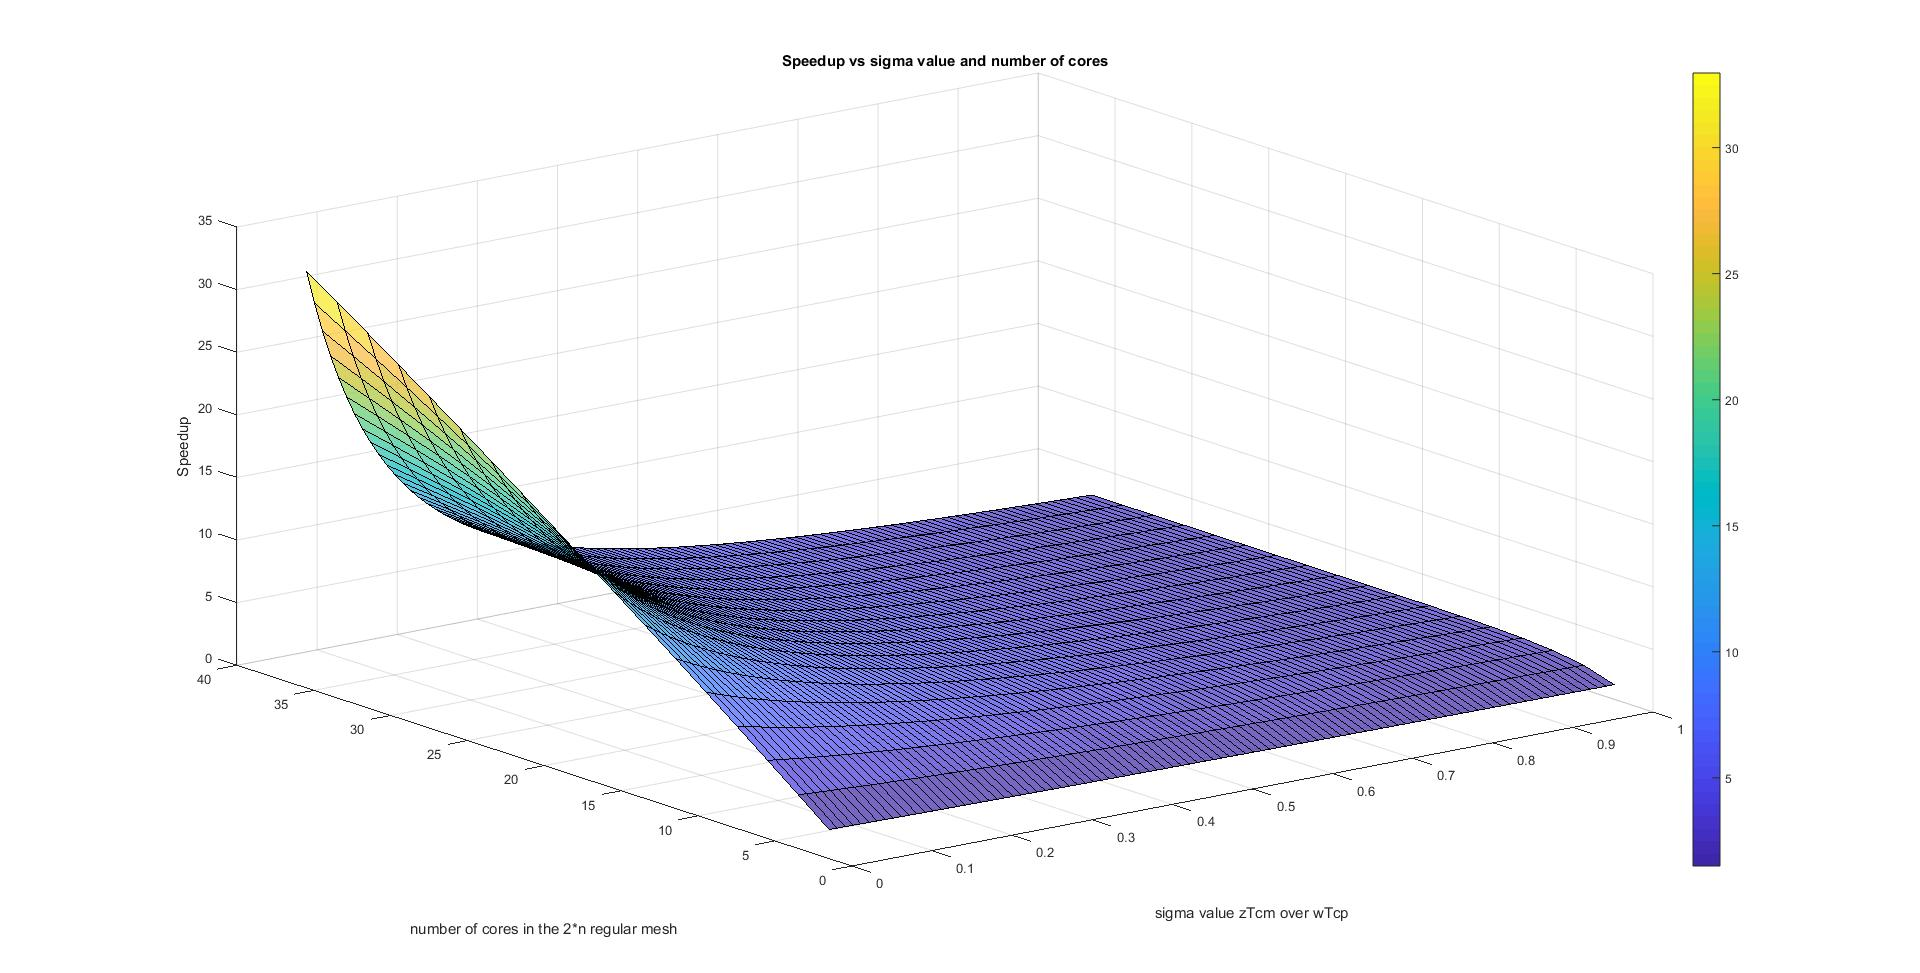
\includegraphics[width=0.85\linewidth]{figure/nocorner2n}
\caption{Speedup vs $\sigma$ value and number of cores in 2*n regular mesh}
\label{nocorner2n}
\end{figure}

\begin{figure}[h]
\centering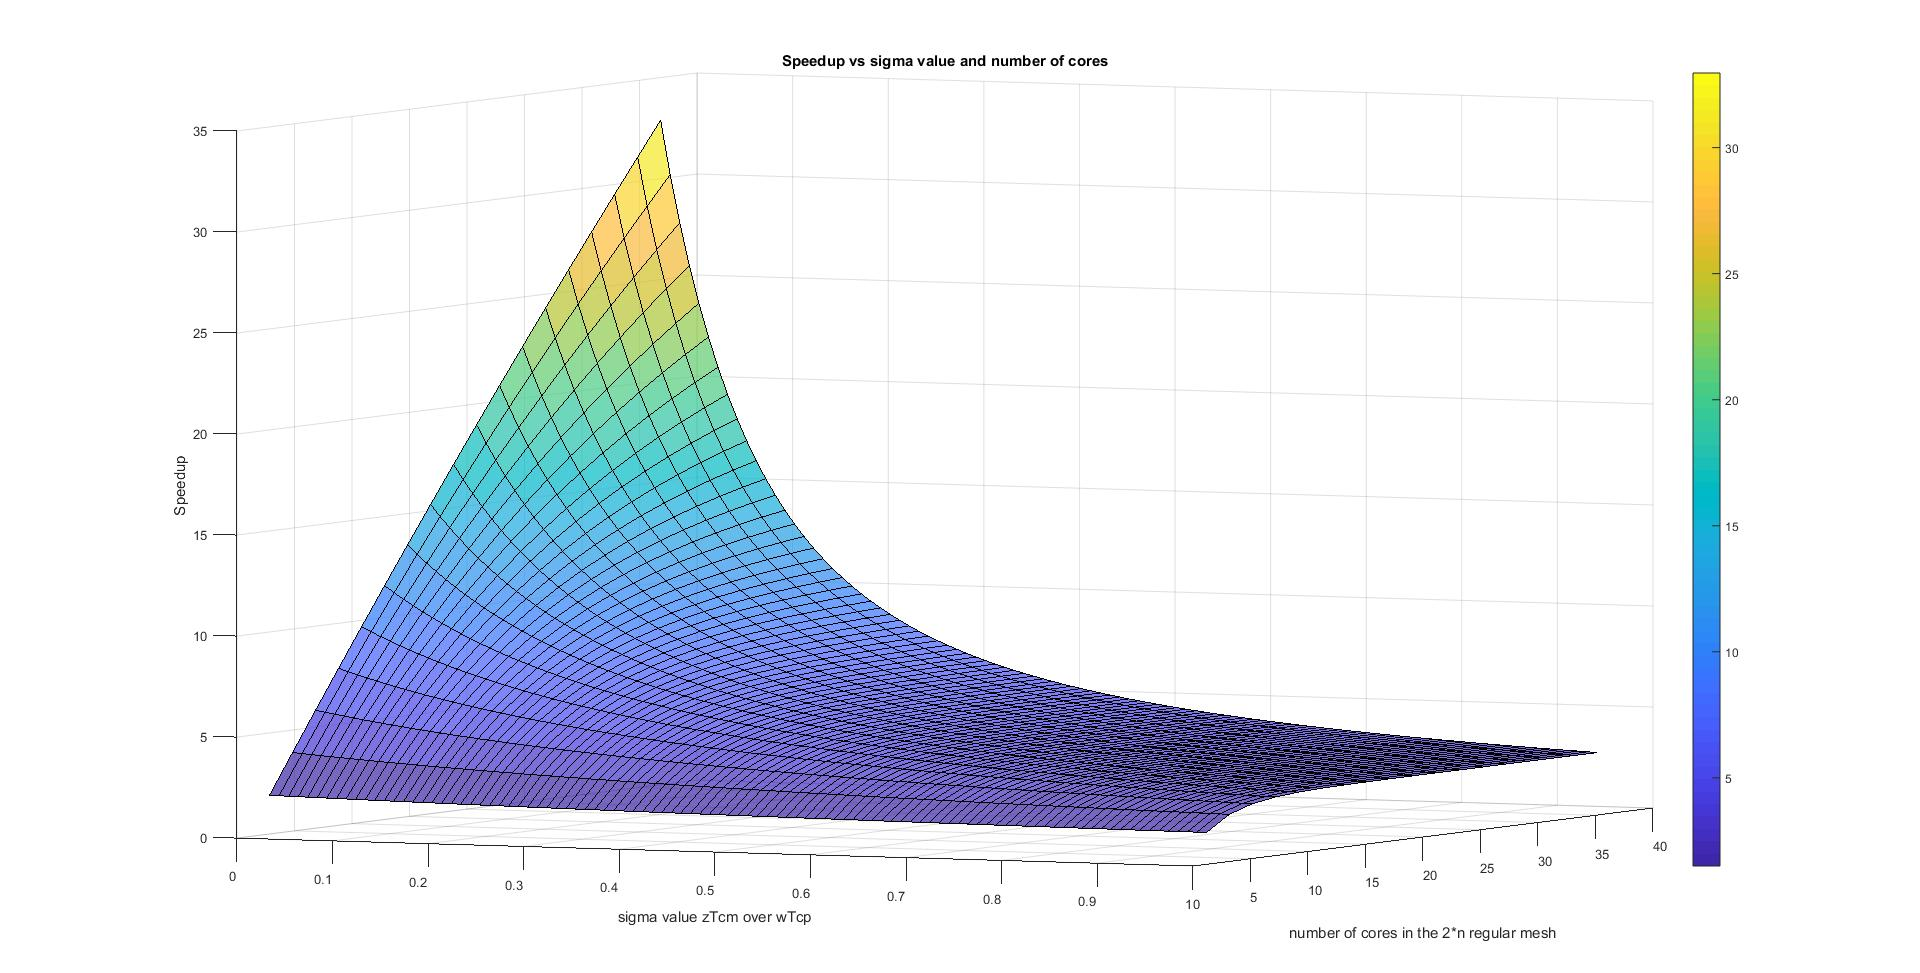
\includegraphics[width=0.85\linewidth]{figure/nocorner2n2}
\caption{Speedup vs $\sigma$ value and number of cores in 2*n regular mesh}
\label{nocorner2n2}
\end{figure}

\vspace*{50pt}

\subsubsection{3*n regular mesh simulation result}

Considering the $3*n $ regular mesh Fig.\ref{38f}.\\

The speedup vs the number of cores relationship as follows:

\begin{itemize}
\item If the $\sigma > 0.2$, the boundary data injection plan has positive speedup effect comparing with the corner injection plan. 
\item If the $\sigma <= 0.2$, the corner data injection plan will play a more helpful role.
\end{itemize}

\begin{figure}[h]
\centering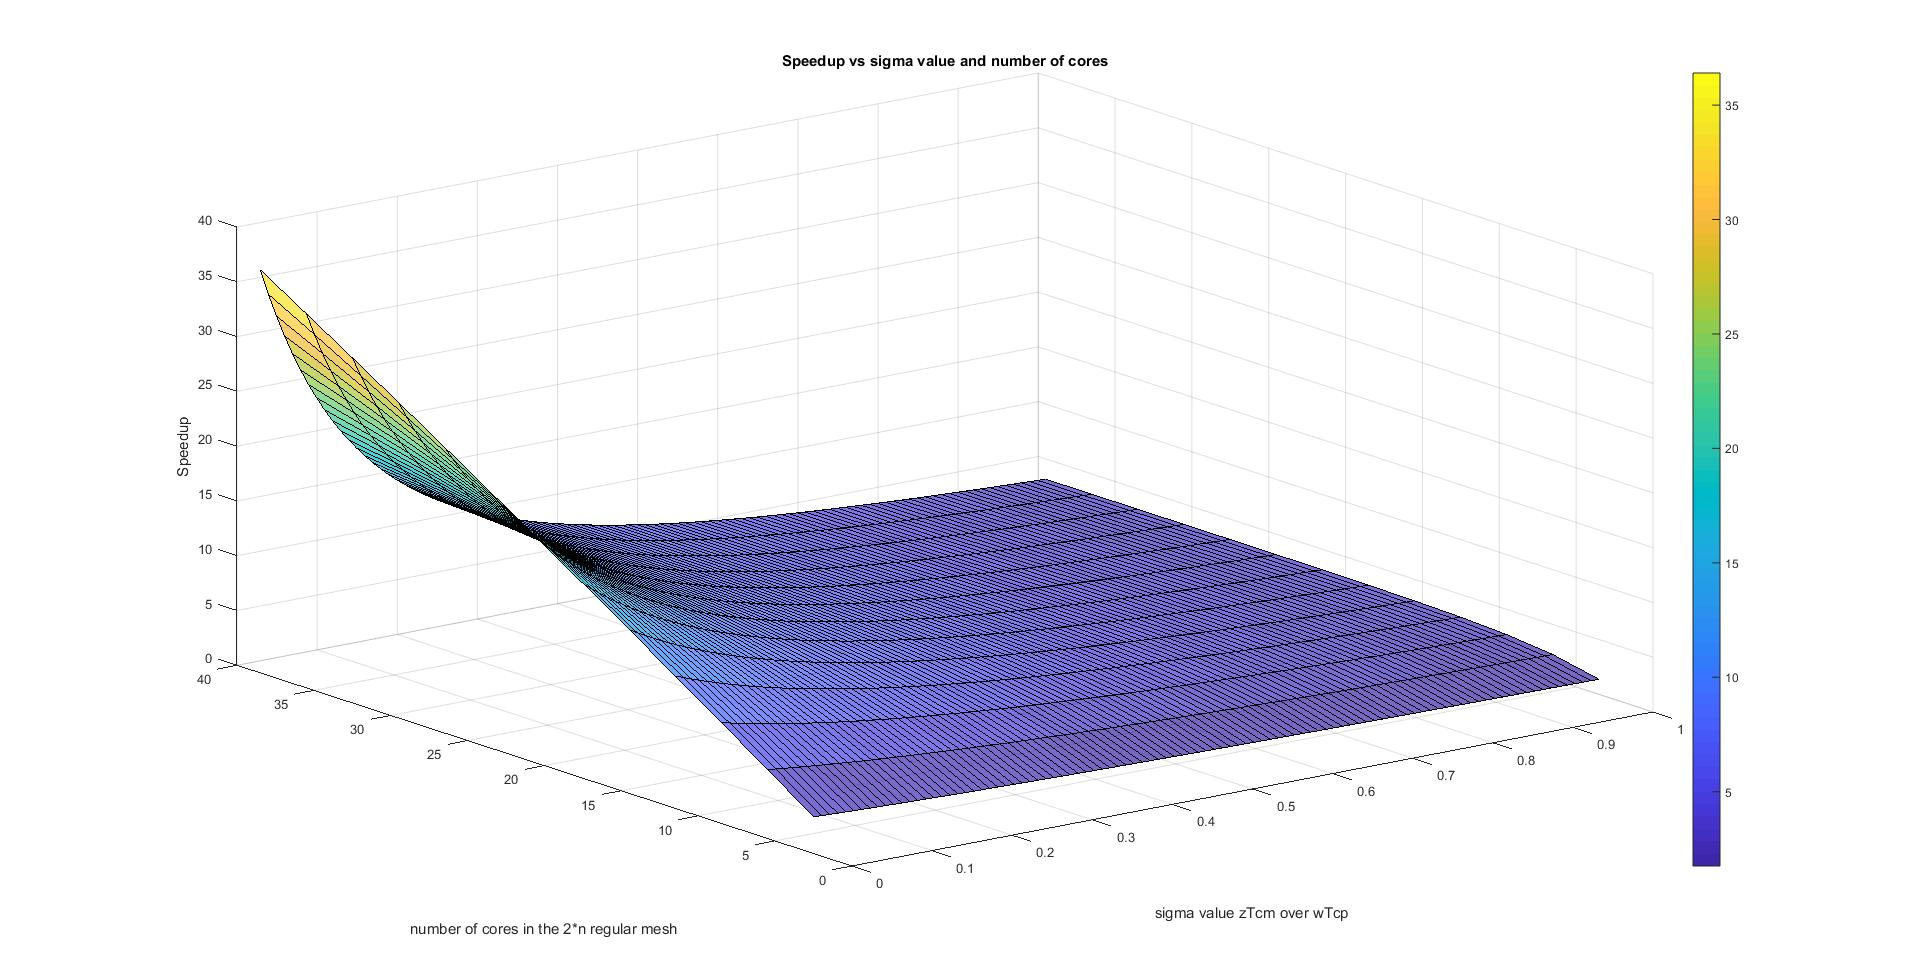
\includegraphics[width=0.85\linewidth]{figure/nocorner3n}
\caption{Speedup vs $\sigma$ value and number of cores in 3*n regular mesh}
\label{nocorner3n}
\end{figure}

\begin{figure}[h]
\centering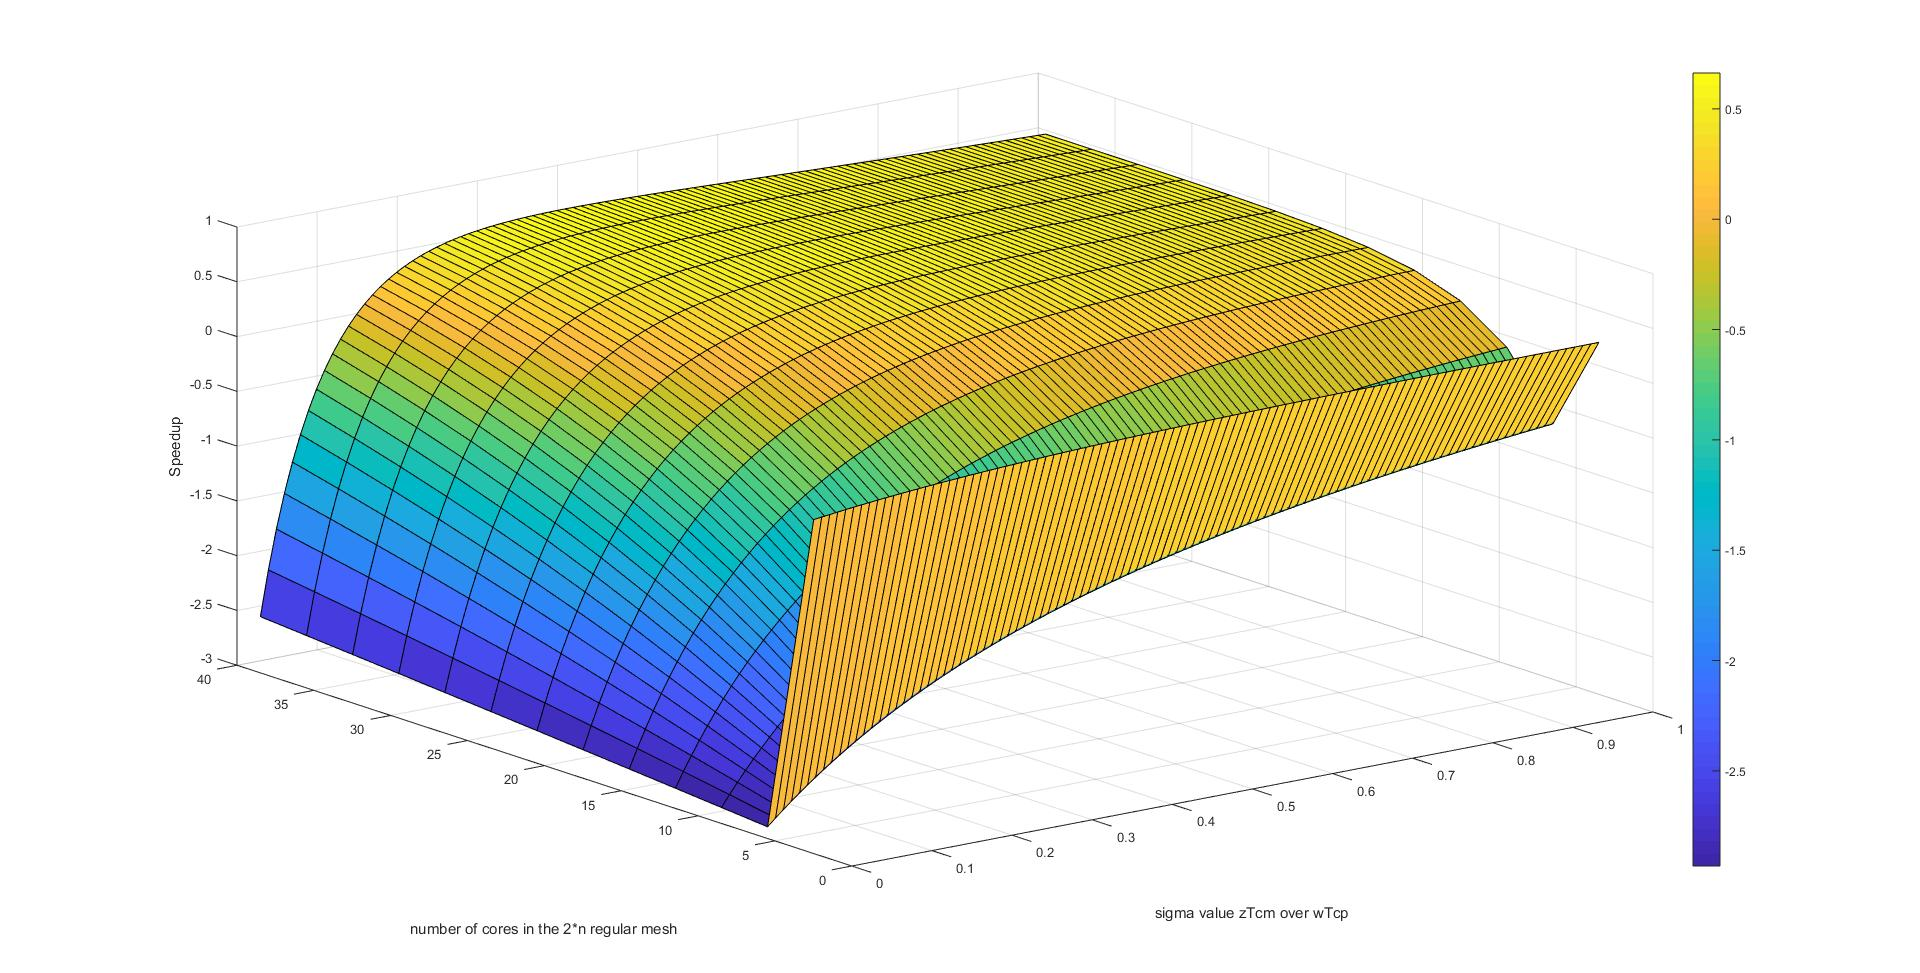
\includegraphics[width=0.85\linewidth]{figure/nobc3n}
\caption{Speedup Difference between Corner and Boundary Data Injection in 3*n regular mesh}
\label{nobc3n}
\end{figure}


\vspace*{50pt}
\subsubsection{5*5 regular mesh inner grid simulation result}
Considering the $5*5 $ regular mesh Fig.\ref{410f} and the data injection position is on the $position = 12$.
\\
The simulation result as follows Fig.\ref{noinner4n}:

\begin{figure}[h]
\centering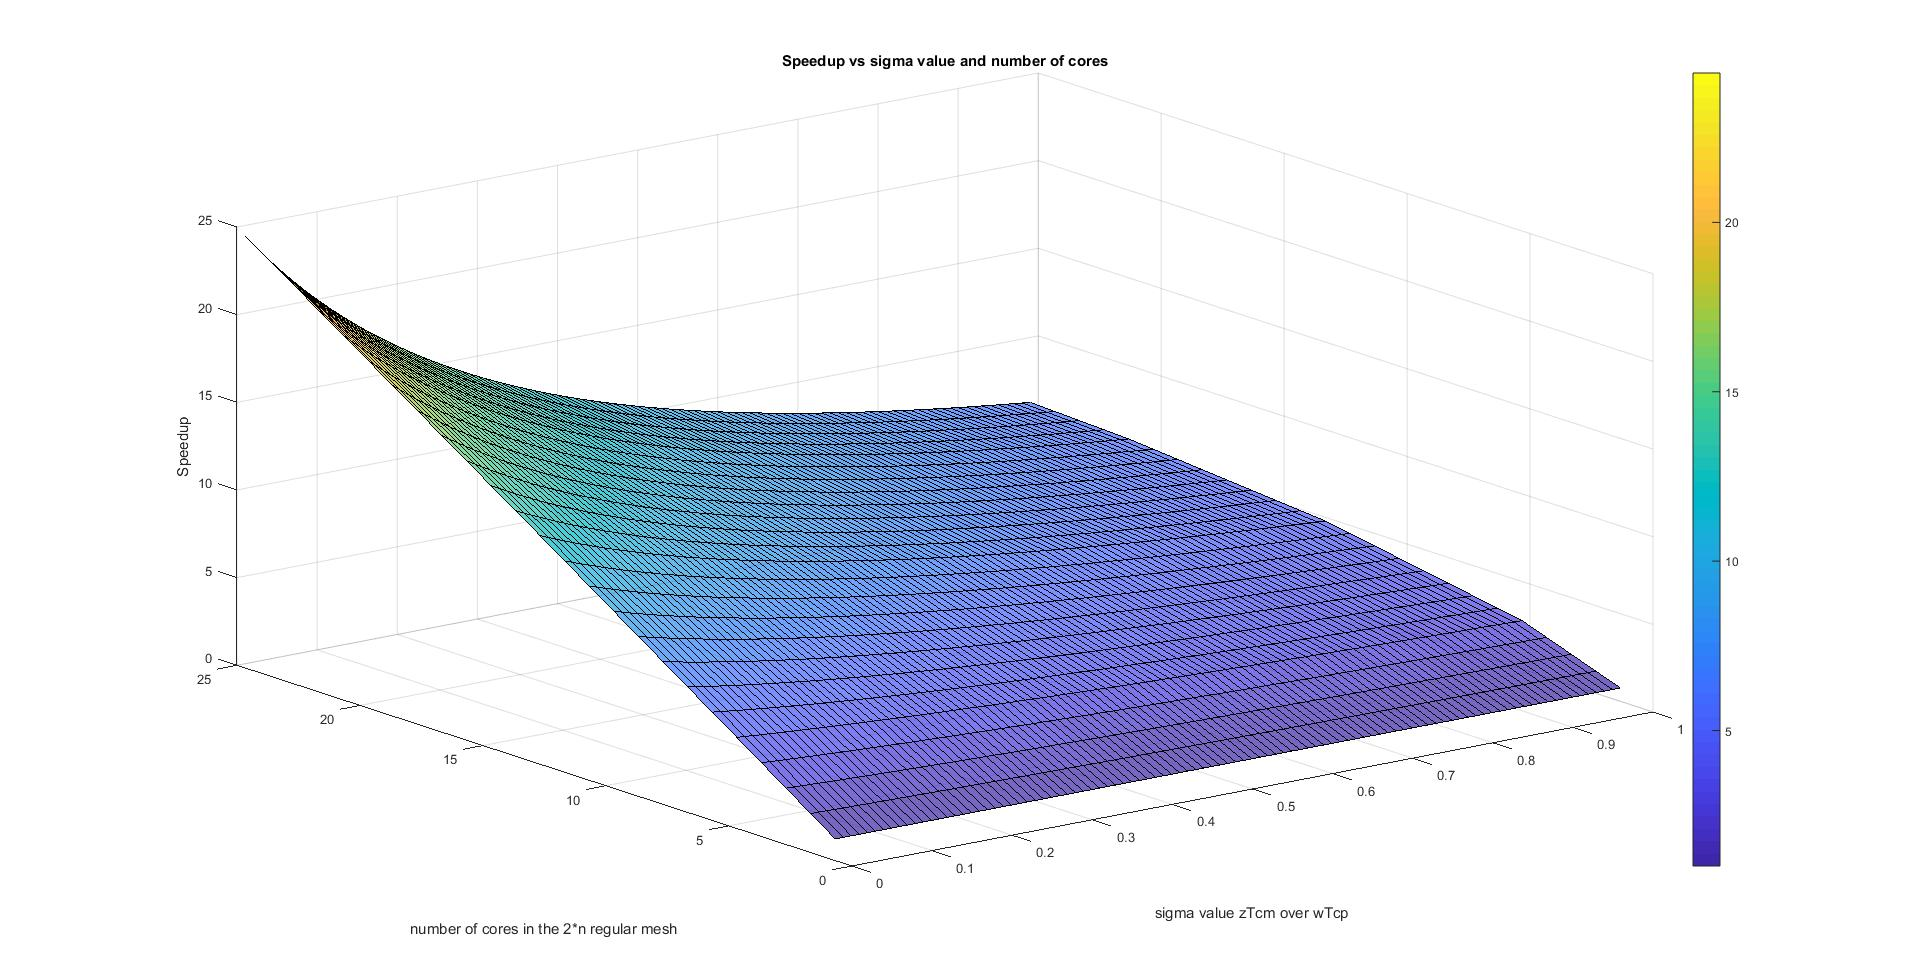
\includegraphics[width=0.85\linewidth]{figure/noinner4n}
\caption{Speedup vs $\sigma$ value and number of cores in 4*n regular mesh}
\label{noinner4n}
\end{figure}
